% SC3010 --- Chapter 2: Cryptographic Tools (0->100 ground-up)
\chapter{Cryptographic Tools: AES, RSA, Hashes and PKI}
\label{ch:crypto}

\begin{quote}
\emph{``Cryptography is not magic---it is mathematics plus careful engineering.''} We turn intuition (locked boxes, fingerprints) into precise tools: symmetric ciphers for speed, asymmetric ciphers for key distribution, hashes for integrity, and PKI for trust at scale.
\end{quote}

\noindent\fbox{\parbox{\dimexpr\linewidth-2\fboxsep-2\fboxrule}{%
\textbf{From zero: high-school arithmetic to real crypto.} We assume no prior cryptography. Start from ``what does it mean to hide a message?'' then formalise encryption, see why one key is not enough, build RSA from modular arithmetic, and end with how your browser trusts a server it has never met.}}
\vspace{0.4em}

\section*{Learning Outcomes}
After this chapter you will be able to:
\begin{enumerate}[label=(L\arabic*)]
    \item explain symmetric encryption and AES structure at a conceptual level;
    \item describe RSA key generation, encryption and decryption and why it works;
    \item state the three hash properties and choose the right one for a task;
    \item construct a certificate chain and verify it to a trust anchor;
    \item select symmetric vs.\ asymmetric vs.\ hash vs.\ PKI for a given requirement.
\end{enumerate}

% ============================================================
\section{Symmetric Encryption and AES}
\label{sec:symmetric}
Intuition: Alice and Bob share one physical key that both locks and unlocks the same box. Anyone with the key can do both. That is \emph{symmetric} encryption: one secret key $k$ for both directions. Formally a scheme is $(\mathsf{Gen},\mathsf{Enc},\mathsf{Dec})$ with $\mathsf{Dec}_k(\mathsf{Enc}_k(m))=m$ and ciphertext reveals nothing about $m$ without $k$.

The one-time pad (Vernam) is perfect: $c = m \oplus k$, $|k|=|m|$, random $k$ used once. Shannon proved it has perfect secrecy, but the key must be as long as the message and never reused---impractical. Modern ciphers trade perfection for efficiency with a short reusable key and computational security.

\textbf{AES} (Advanced Encryption Standard) is the standard symmetric cipher: block size 128 bits, key 128/192/256 bits, 10/12/14 rounds. Each round is a substitution--permutation network:

\begin{figure}[h]
\centering
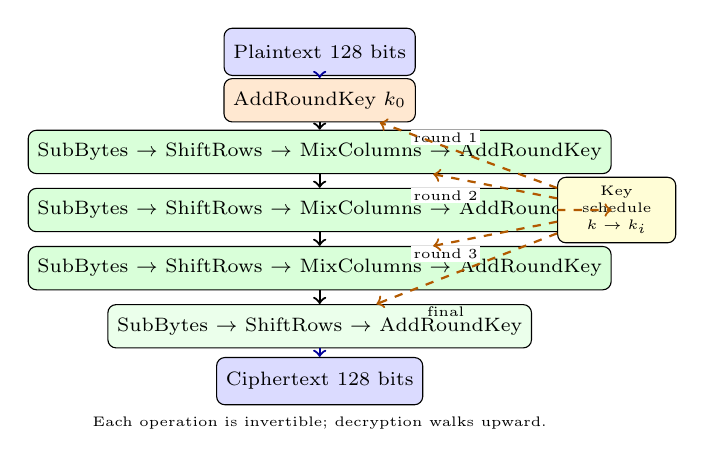
\begin{tikzpicture}[scale=0.82,every node/.style={font=\scriptsize}]
  \node[draw,fill=blue!14,rounded corners=3pt,minimum width=2.2cm,minimum height=0.6cm] (pt) at (0,3.0) {Plaintext 128 bits};
  \node[draw,fill=orange!18,rounded corners=3pt,minimum width=2.2cm,minimum height=0.55cm] (ak0) at (0,2.25) {AddRoundKey $k_0$};
  \foreach \i/\y in {1/1.45,2/0.55,3/-0.35} {
    \node[draw,fill=green!15,rounded corners=3pt,minimum width=3.4cm,minimum height=0.55cm] (r\i) at (0,\y) {SubBytes $\to$ ShiftRows $\to$ MixColumns $\to$ AddRoundKey};
    \node[font=\tiny,fill=white,inner sep=1pt] at (1.95,\y+0.22) {round \i};
  }
  \node[draw,fill=green!8,rounded corners=3pt,minimum width=3.4cm,minimum height=0.55cm] (rf) at (0,-1.25) {SubBytes $\to$ ShiftRows $\to$ AddRoundKey};
  \node[font=\tiny] at (1.95,-1.03) {final};
  \node[draw,fill=blue!14,rounded corners=3pt,minimum width=2.2cm,minimum height=0.6cm] (ct) at (0,-2.1) {Ciphertext 128 bits};
  \draw[->,thick,blue!60!black] (pt) -- (ak0);
  \draw[->,thick] (ak0) -- (r1); \draw[->,thick] (r1) -- (r2); \draw[->,thick] (r2) -- (r3); \draw[->,thick] (r3) -- (rf); \draw[->,thick,blue!60!black] (rf) -- (ct);
  \node[draw,fill=yellow!16,rounded corners=3pt,minimum width=1.5cm,align=center,font=\tiny] (keys) at (4.6,0.55) {Key\\schedule\\$k\to k_i$};
  \draw[->,thick,orange!70!black,dashed] (keys) -- (ak0); \draw[->,thick,orange!70!black,dashed] (keys) -- (r1);
  \draw[->,thick,orange!70!black,dashed] (keys) -- (r2); \draw[->,thick,orange!70!black,dashed] (keys) -- (r3); \draw[->,thick,orange!70!black,dashed] (keys) -- (rf);
  \node[font=\tiny,align=center] at (0,-2.75) {Each operation is invertible; decryption walks upward.};
\end{tikzpicture}
\caption{AES round structure (128-bit key, 10 rounds shown schematically). SubBytes adds non-linearity, ShiftRows and MixColumns diffuse bits, AddRoundKey mixes the key. Repetition gives confusion and diffusion.}
\label{fig:aes}
\end{figure}

Confusion (SubBytes) hides the relation between key and ciphertext; diffusion (ShiftRows + MixColumns) spreads one plaintext bit over many ciphertext bits. Repeating 10--14 times makes the cipher look random without the key.

AES encrypts blocks; long messages need a \emph{mode}. ECB (each block independently) leaks patterns and must be avoided. Use \textbf{CBC} or \textbf{CTR} with a random IV, or better \textbf{GCM} (CTR plus authentication). GCM provides \emph{authenticated encryption}: confidentiality and integrity together. Never invent your own mode.

The hard part is not AES itself but \emph{key distribution}: how do Alice and Bob share $k$ without meeting? Sending $k$ in the clear defeats the purpose. We need a second tool.

\begin{lstlisting}[language=Python,caption={AES-GCM encrypt/decrypt (conceptual; use a real library).},label={lst:aesgcm}]
from cryptography.hazmat.primitives.ciphers.aead import AESGCM
import os
key = AESGCM.generate_key(bit_length=128)   # 16 bytes, keep secret
aesgcm = AESGCM(key)
nonce = os.urandom(12)                       # 96-bit, never reuse with same key
ct = aesgcm.encrypt(nonce, b"hello SC3010", associated_data=None)
pt = aesgcm.decrypt(nonce, ct, associated_data=None)  # raises if tampered
assert pt == b"hello SC3010"
\end{lstlisting}

% ============================================================
\section{Asymmetric Encryption and RSA}
\label{sec:rsa}
Intuition: a mailbox with an open slot (public key) anyone can drop letters into, but only the owner with the private key can open. \emph{Asymmetric} (public-key) encryption uses a key pair $(pk,sk)$: $pk$ encrypts, $sk$ decrypts. No prior shared secret needed.

\textbf{RSA} (Rivest--Shamir--Adleman, 1977) rests on modular arithmetic. Recall $a \equiv b \pmod n$ means $n\mid(a-b)$, and $\gcd(a,n)=1$ implies $a$ has an inverse modulo $n$.

\begin{definition}[RSA]
Generate two distinct large primes $p,q$, set $n=pq$, $\phi(n)=(p-1)(q-1)$. Choose $e$ with $\gcd(e,\phi(n))=1$, compute $d\equiv e^{-1}\pmod{\phi(n)}$. Public key $pk=(n,e)$, private key $sk=(n,d)$. Encryption of $m\in[0,n)$:
\begin{align}
c \equiv m^{e} \pmod n,
\label{eq:rsa-enc}
\end{align}
decryption:
\begin{align}
m \equiv c^{d} \pmod n.
\label{eq:rsa-dec}
\end{align}
\end{definition}

Why does it work? Euler's theorem: if $\gcd(m,n)=1$, $m^{\phi(n)}\equiv1\pmod n$. Since $ed\equiv1\pmod{\phi(n)}$, write $ed=1+k\phi(n)$. Then
\begin{align}
c^{d} \equiv (m^{e})^{d} = m^{ed} = m^{1+k\phi(n)} = m\cdot(m^{\phi(n)})^{k} \equiv m\cdot1^{k} \equiv m \pmod n.
\end{align}
With Chinese remainder handling for $\gcd(m,n)\neq1$ the same holds. Security rests on hardness of \emph{factoring} $n$ to recover $\phi(n)$ and $d$; with 2048-bit $n$, factoring is infeasible today.

\begin{theorem}[RSA correctness]
For every $m\in\mathbb{Z}_n$, $\mathsf{Dec}_{sk}(\mathsf{Enc}_{pk}(m))=m$ when keys are generated as above.
\end{theorem}

RSA is slow (modular exponentiation of huge numbers) and malleable without padding. Never use textbook RSA. Use \textbf{OAEP} padding for encryption and \textbf{PSS} for signatures, or better use hybrid encryption: RSA (or Diffie--Hellman) to transport a random AES key, then AES for bulk data.

\begin{lstlisting}[language=Python,caption={RSA toy (small primes) --- do not use for real secrecy.},label={lst:rsa}]
import math
p, q = 61, 53
n = p * q
phi = (p-1)*(q-1)
e = 17  # coprime to phi
d = pow(e, -1, phi)  # Python 3.8+: modular inverse
def enc(m): return pow(m, e, n)
def dec(c): return pow(c, d, n)
assert dec(enc(42)) == 42
print(f"n={n} phi={phi} e={e} d={d}")  # n=3233 d=2753
\end{lstlisting}

Key sizes: RSA-2048 $\approx$ 112-bit symmetric security; RSA-3072 $\approx$ 128-bit. For new systems prefer elliptic-curve (ECDH/ECDSA) or post-quantum KEMs where available---same ideas, smaller keys.

% ============================================================
\section{Cryptographic Hashes}
\label{sec:hash}
A hash is a fingerprint: arbitrary input $\to$ fixed output, easy to compute, hard to invert. Formally $H:\{0,1\}^*\to\{0,1\}^n$ with $n=256$ for SHA-256.

\begin{figure}[h]
\centering
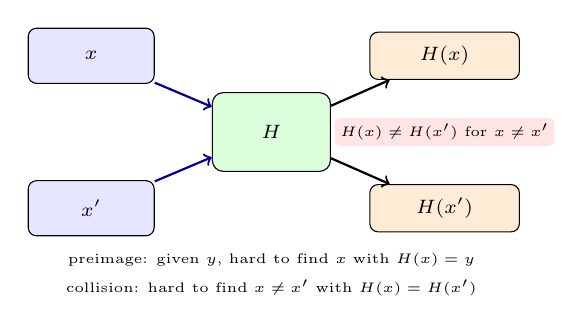
\begin{tikzpicture}[scale=0.88,every node/.style={font=\scriptsize}]
  \node[draw,fill=blue!10,rounded corners=3pt,minimum width=1.6cm,minimum height=0.7cm,align=center] (a) at (0,1.1) {$x$};
  \node[draw,fill=blue!10,rounded corners=3pt,minimum width=1.6cm,minimum height=0.7cm,align=center] (b) at (0,-1.1) {$x'$};
  \node[draw,fill=green!14,rounded corners=4pt,minimum width=1.5cm,minimum height=1.0cm,align=center] (h) at (2.6,0) {$H$};
  \node[draw,fill=orange!16,rounded corners=3pt,minimum width=1.9cm,minimum height=0.6cm,align=center] (ha) at (5.1,1.1) {$H(x)$};
  \node[draw,fill=orange!16,rounded corners=3pt,minimum width=1.9cm,minimum height=0.6cm,align=center] (hb) at (5.1,-1.1) {$H(x')$};
  \draw[->,thick,blue!60!black] (a) -- (h); \draw[->,thick,blue!60!black] (b) -- (h);
  \draw[->,thick] (h) -- (ha); \draw[->,thick] (h) -- (hb);
  \node[font=\tiny,fill=red!10,rounded corners=2pt,inner sep=2pt] at (5.1,0) {$H(x)\neq H(x')$ for $x\neq x'$};
  \node[font=\tiny,align=left] at (2.6,-1.85) {preimage: given $y$, hard to find $x$ with $H(x)=y$};
  \node[font=\tiny,align=left] at (2.6,-2.25) {collision: hard to find $x\neq x'$ with $H(x)=H(x')$};
\end{tikzpicture}
\caption{Hash properties visualised. Even one-bit change avalanches the digest; finding any preimage or collision should be infeasible ($2^{256}$ work for SHA-256).}
\label{fig:hash}
\end{figure}

\begin{definition}[Hash security]
$H$ is (a) \textbf{preimage resistant} if given $y$ it is hard to find $x$ with $H(x)=y$; (b) \textbf{second-preimage resistant} if given $x$ it is hard to find $x'\neq x$ with $H(x')=H(x)$; (c) \textbf{collision resistant} if hard to find \emph{any} $x\neq x'$ with $H(x)=H(x')$. Collision resistance implies second-preimage resistance.
\end{definition}

Applications: file integrity ($H(\text{file})$ detects tampering), password storage (store salted slow hash, not plaintext), commitments, Merkle trees for blockchains. For integrity \emph{with a key}, use \textbf{HMAC}: $\text{HMAC}_k(m)=H((k\oplus\text{opad})\Vert H((k\oplus\text{ipad})\Vert m))$, or an AEAD mode directly.

Birthday bound: collisions for $n$-bit hash need $\approx2^{n/2}$ work by the birthday paradox, so SHA-256 gives 128-bit collision security. MD5 and SHA-1 are broken for collisions---do not use.

\begin{lstlisting}[language=Python,caption={SHA-256 and HMAC.},label={lst:hash}]
import hashlib, hmac
msg = b"SC3010 is fun"
print(hashlib.sha256(msg).hexdigest())
# hmac with a secret key
key = b"secret-key-16bytes"
tag = hmac.new(key, msg, hashlib.sha256).hexdigest()
# verify by recomputing and comparing with hmac.compare_digest
assert hmac.compare_digest(tag, hmac.new(key, msg, hashlib.sha256).hexdigest())
\end{lstlisting}

% ============================================================
\section{Hybrid Encryption and Key Exchange}
\label{sec:hybrid}
In practice we never choose one tool alone. \textbf{Hybrid encryption} uses asymmetric crypto to transport a fresh symmetric key, then symmetric crypto for bulk data---combining key-distribution without a shared secret with AES speed.

\textit{Bulk via AES, key via RSA/ECDH.} Sender picks random $k\gets\{0,1\}^{128}$, computes $c_1=\mathsf{Enc}_{pk}(k)$ with RSA-OAEP or ECIES, $c_2=\mathsf{Enc}^{\text{AES-GCM}}_k(m)$, sends $(c_1,c_2)$. Receiver recovers $k=\mathsf{Dec}_{sk}(c_1)$ then $m$. Even if $m$ is gigabytes, only 256 bytes use slow public-key work.

\textbf{Diffie--Hellman (DH)} offers an alternative without encryption: Alice picks $a$, sends $g^a\bmod p$; Bob picks $b$, sends $g^b\bmod p$; both compute $g^{ab}\bmod p$ as the shared secret. An eavesdropper sees $g^a,g^b$ but not $g^{ab}$ (discrete-log hardness). DH needs authentication---otherwise a man-in-the-middle substitutes both sides---so it is paired with signatures or PKI (next section). Modern TLS 1.3 uses ephemeral ECDH (curve P-256 or X25519) for forward secrecy: even if the long-term key leaks later, past $g^{ab}$ values remain secret because $a,b$ were ephemeral.

\begin{definition}[Forward secrecy]
A key-exchange has \textbf{forward secrecy} if compromise of long-term keys does not reveal past session keys. Ephemeral DH/ECDH provides it; static RSA key transport does not.
\end{definition}

\begin{example}[Why hybrid matters]
Encrypting a 10\,MB video with RSA-2048 directly would need $>40{,}000$ RSA blocks and minutes of CPU. Hybrid does one RSA operation (milliseconds) plus 10\,MB of AES-GCM at gigabytes per second. Use the right tool for each job.
\end{example}

% ============================================================
\section{Public-Key Infrastructure (PKI)}
\label{sec:pki}
Asymmetric crypto solves key distribution but creates a new question: whose public key is this? Without binding, an attacker substitutes their own $pk$. PKI binds names to keys via certificates.

A \textbf{certificate} is $\text{Cert}=\langle \text{subject}, pk_{\text{subject}}, \text{validity}, \text{issuer}, \text{extensions}, \sigma\rangle$ where $\sigma = \mathsf{Sign}_{sk_{\text{issuer}}}(H(\text{rest}))$. A \textbf{Certificate Authority (CA)} is an entity trusted to issue and revoke certificates. Your device ships with a \emph{trust store} of root CA public keys (trust anchors).

\begin{figure}[h]
\centering
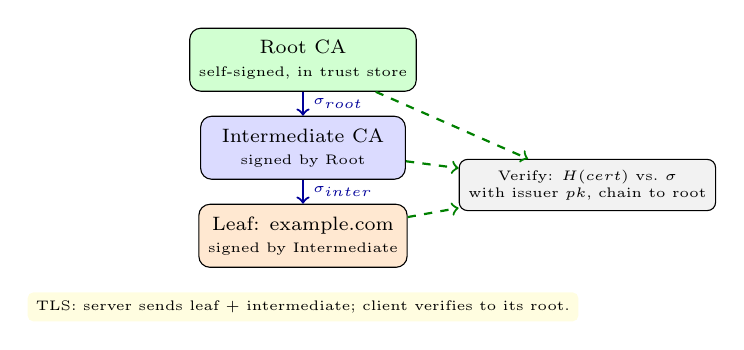
\begin{tikzpicture}[scale=0.86,every node/.style={font=\scriptsize}]
  \node[draw,fill=green!18,rounded corners=4pt,minimum width=2.6cm,minimum height=0.8cm,align=center] (root) at (0,2.4) {Root CA\\\tiny self-signed, in trust store};
  \node[draw,fill=blue!14,rounded corners=4pt,minimum width=2.6cm,minimum height=0.8cm,align=center] (inter) at (0,1.1) {Intermediate CA\\\tiny signed by Root};
  \node[draw,fill=orange!18,rounded corners=4pt,minimum width=2.6cm,minimum height=0.8cm,align=center] (leaf) at (0,-0.2) {Leaf: example.com\\\tiny signed by Intermediate};
  \draw[->,thick,blue!60!black] (root) -- (inter) node[midway,right,font=\tiny] {$\sigma_{\text{root}}$};
  \draw[->,thick,blue!60!black] (inter) -- (leaf) node[midway,right,font=\tiny] {$\sigma_{\text{inter}}$};
  \node[draw,fill=gray!10,rounded corners=3pt,minimum width=3.0cm,minimum height=0.65cm,align=center,font=\tiny] (verify) at (4.2,0.55) {Verify: $H(\text{cert})$ vs.\ $\sigma$\\with issuer $pk$, chain to root};
  \draw[->,thick,green!50!black,dashed] (leaf) -- (verify);
  \draw[->,thick,green!50!black,dashed] (inter) -- (verify);
  \draw[->,thick,green!50!black,dashed] (root) -- (verify);
  \node[font=\tiny,align=center,fill=yellow!12,rounded corners=2pt,inner sep=3pt] at (0,-1.25) {TLS: server sends leaf + intermediate; client verifies to its root.};
\end{tikzpicture}
\caption{Certificate chain of trust. Each certificate is signed by its issuer; verification walks upward until a trust anchor. Revocation via CRL/OCSP prunes broken links.}
\label{fig:pki}
\end{figure}

Verification: given leaf for \texttt{example.com}, fetch intermediate, verify $\sigma_{\text{inter}}$ on leaf with $pk_{\text{inter}}$, then verify $\sigma_{\text{root}}$ on intermediate with $pk_{\text{root}}$ from trust store, check validity periods, name matches, and revocation (CRL or OCSP). If all pass, $pk_{\text{leaf}}$ is trusted for that name. TLS (HTTPS) does exactly this during the handshake before any AES session key is negotiated.

Threats to PKI: CA compromise, mis-issuance, name-constraint bypass, revoked-but-still-trusted certs. Mitigations include Certificate Transparency (public logs of all certs), short-lived certs, OCSP stapling, and pinning.

\begin{example}[What PKI does not solve]
PKI authenticates the \emph{server name}, not that the server is honest. A valid certificate for \texttt{evil-phishing.example} passes PKI but the site still steals passwords. Users must also check the name matches their intent---hence EV deprecation and browser warnings for look-alike domains (homograph attacks). PKI is necessary but not sufficient; user education and allow-lists matter too.
\end{example}

\begin{remark}[Key management in practice]
Generate keys in an HSM or OS keystore, never hard-code them; rotate regularly; back up the private key securely or accept that loss means re-issuance; use ACME (Let's Encrypt) to automate short-lived certificates and avoid expiry outages that still top outage post-mortems every year.
\end{remark}

% ============================================================
\section{Chapter Notes}
For AES internals see Daemen and Rijmen, \emph{The Design of Rijndael}; for modes and AEAD see NIST SP 800-38A/D. RSA is from Rivest, Shamir, Adleman (1978); textbook vs.\ padded RSA is covered in Katz and Lindell, \emph{Introduction to Modern Cryptography}. Hash functions: NIST FIPS 180-4 (SHA-2) and 202 (SHA-3). PKI and TLS: RFC 5280 (certificates) and RFC 8446 (TLS 1.3); Shostack and Gutmann give practitioner views. For post-quantum migration see NIST PQC standards (2024).

% ============================================================
\section{Exercises}
\label{sec:ch02-exercises}
\begin{enumerate}[label=E2.\arabic*, leftmargin=*, itemsep=0.8em]
    \item \textbf{AES and modes.} Why does AES-ECB leak plaintext patterns? Sketch a $2\times2$ pixel image where ECB preserves the outline. Which mode(s) would you recommend for (a) disk encryption with random access and (b) a TLS record layer, and why?
    \item \textbf{RSA by hand.} Let $p=17$, $q=23$, $e=5$. Compute $n$, $\phi(n)$, $d$, then encrypt $m=42$ and decrypt. Show Euler step $ed=1+k\phi(n)$ explicitly. What goes wrong if you reuse $n$ with two different $e$ values across users?
    \item \textbf{Hash properties.} Order the three hash properties by strength (which implies which). Give an application that needs only second-preimage resistance but not collision resistance, and one that needs collision resistance. Explain why MD5 is unsafe for signatures even if preimage still seems hard.
    \item \textbf{HMAC vs.\ plain hash.} Why is $\text{HMAC}_k(m)$ preferred over $H(k\Vert m)$ for message authentication? Describe a length-extension attack on SHA-256 and how HMAC defeats it. When would you use HMAC versus AES-GCM?
    \item \textbf{PKI verification.} A browser receives leaf for \texttt{shop.example} signed by Inter-CA, which is signed by Root R in its trust store. List the five checks the browser performs before showing a padlock. An attacker compromises Inter-CA but not Root---what can they forge, and how do CT logs and OCSP help detect and contain it?
\end{enumerate}
% End of Chapter 2
